\documentclass{report}
\usepackage[T1]{fontenc}
\usepackage[utf8]{inputenc}
\usepackage{lmodern}
\usepackage[numbers]{natbib}
\usepackage{amsthm}
\usepackage{amsmath}
\usepackage{graphicx}

\title{Stock Market Prediction}
\author{Mark Dunne}

\begin{document}

\maketitle
\tableofcontents

\begin{abstract}

This project is an attempt to answer the question of whether stock market prices can be accurately predicted using modern Artificial Techniques. We take multiple approaches to the problem including Fundamental Analysis, Technical Analysis, and Machine Learning techniques.

\end{abstract}

\section{Introduction}
\subsection{Introduction}
\subsection{Project motivation}
\subsection{Importance and prevalence of the problem}
Explain size of the financial industry affected by the problem and why having better tools to predict the stock market may be important to the average person

\subsection{Project goals}

\subsection{Project outline}
How the project will meet those goals

\section{Background}
\subsection{The Stock Market}
\subsubsection{What is the stock market}
\subsubsection{How the stock market works}
\subsubsection{Components of the stock market}
\subsubsection{Terminology}

Fundamental analysis

\subsubsection{The Efficient Market Hypothesis}

Throughout this area of investigation, there is a very large elephant in the room, the Efficient Market Hypothesis (EMH). The hypothesis talks specifically about an agents ability to profit from make inefficiencies, i.e when stocks and shares are mispriced by the market. Its strongest proponents would claim that the very title of this report, predicting stock market, is all but impossible. The EMH comes in three main forms.
\begin{itemize}
  \item The weak form of the efficient market hypothesis claims that prices fully
reflect the information implicit in the sequence of past prices. 

  \item The semi-strong form of the hypothesis asserts that prices reflect all relevant information that is publicly available
  
  \item the strong form of market efficiency asserts information that is known to any participant is reflected in market prices.
\end{itemize}
\cite{dimson1998brief}

Informally, the weak form implies that you cannot profit using historical patterns in the share price, the semi-strong form implies that there is profit only to be made from insider trading, and the strong form says that even this is futile. Important to note is that the week form the the hypothesis does not completely rule out profitable trading on the stock market. Trading profitably based on predictions from Fundamental analysis is still possible in the week form. 

Clearly for the successful application of modern AI techniques to this problem, we must hope that at least the semi-strong and strong forms of the hypothesis are wrong and do allow for a sufficiently intelligent agent to profit. Luckily, many researchers do indeed question the validity of the hypothesis. There is evidence that the stock market does not always follow EMH. \citet{basu1983relationship} showed that fundamental analysis could yeild information useful in future market forecasts. This result questions the semi-strong and strong forms of the hypothesis, but does not necessarily break the weak form. 

Later in this report, we provide our own data and analysis that supports the view that at most only the week form of the EMH holds true.

\subsection{Analysis of the problem}
\subsubsection{Explanation of the difficulty of the problem}
\subsubsection{Separation of profitability and accuracy}
\subsubsection{Temporal reach of prediction}

Want to avoid HFT

Fundamental is long term

Machine learning focus on short/medium

\subsubsection{Formal definition of the problem}

\subsection{Review of existing work}

\section{Methodology and Data}
\subsection{Tools Used}
\subsubsection{Python and associated packages}

Python was the language of choice for this project. This was an easy decision for the following reasons.

\begin{enumerate}
  \item Python as a language has an enourmous community behind it. Any problems that might be encountered on the way can be easily solved with a trip to Stack Overflow. Python is amoung the most popular languages on the site which makes it very likely there will be a direct answer to any query \cite{website:redmonk-languages}. 
  
  \item Python has an abundance of powerful tools ready for scientific computing. Packages such as Numpy, Pandas, and SciPy are freely available, performant and well documented. Packages such as these can dramatically reduce and simplify the code needed to write a given program. This makes iteration quick.

  \item Python as a language is forgiving and allows for programs that look like pseudo code. This is useful when pseudo code given in academic papers needs to be implemented and tested. Using Python, this step is usually reasonably trivial.

\end{enumerate}


However, I digress, Python is not without its flaws. The language is dynamically typed and packages are notorious for Duck Typing. This can be frustrating when a package method returns something that, for example, looks like an array rather than being an actual array. Coupled with the fact that standard Python documentation does not explicitly state the return type of a method, this can lead to a lot of trial and error type testing that would not otherwise happen in a strongly typed language such as Haskell. In my view, this is an issue that makes learning to use a new Python package more difficult than it otherwise could be.\newline


\noindent The following packages were used throughout the project

\begin{description}

  \item[Numpy] \hfill \\ A staple of scientific computing, useful for efficient data structures and linear algebra.
   
  \item[Pandas] \hfill \\ Useful for filtering and mutating the data into a desired form.  
  
  \item[SciPy] \hfill \\ Extensive library of numerical routines
  
  \item[Matplotlib] \hfill \\ Used for graphing data

\end{description}  
 
  
\subsubsection{Quantopian/Zipline and Pyalgotrade}
\subsubsection{Statsmodels}

\subsection{Data Used}
\subsubsection{Data sources}
\subsubsection{Format of the data}
\subsubsection{Adjusted prices}

\subsection{Simulation of strategies}
Similarity to real life

\subsection{Defining a successful model}
Statistical significance of a model

\section{Attacking the problem - Fundamental Analysis}

We begin by approaching the problem using Fundamental Analysis. 

Fundamental Analysis of stocks and shares is one of the earliest and forms of market prediction. It takes the view that the market has mispriced a security, but over time the price will be corrected to its intrinsic value. If we can accurately calculate the intrinsic value of a security, e.g how much is one share of company \textit{X} actually worth, then we can choose to invest based on the difference between the current price and intrinsic value. 

\citet{graham1934security} laid the groundwork for the field with the book \textit{Security Analysis}. He encouraged would-be investors to estimate the intrinsic value of a stock before buying or selling based on trends, a novel idea at the time. It stands as testament to his approach that his only A+ student was Warren Buffet who methodically applied the strategy and has enjoyed renowned success since. \cite{schroeder2008snowball}

\subsection{P/E Ratio}

One of the simplest and possible most well known approach to gauging the intrinsic value of a stock is to use the P/E Ratio. P/E Ratio is defined as follows\\

\begin{math}
	\text{P/E Ratio} = \dfrac{\text{Share Price}}{\text{Earnings Per Share}}
\end{math}\\

The intuition on why this metric might be used is that if the ratio is high, it means that investors are willing to pay more for every dollar the company earns; they have more faith in the company. For example, if a company is trading at \$20, and the Earnings Per Share is \$100, then the P/E Ratio is 5. This translates to the investor willing to pay \$5 for every dollar of the company's earnings.Although simplistic in nature, we were able to achieve surprising results based on this ratio. 

We analysed 497 companies in the S&P index from 1990 to 2014 and compared their P/E Ratio to the change in their stock price the following year. If the P/E Ratio is indicative of future performance, we should see larger, positive, changes in the stock price of companies with a high PE Ratio compared to those with a lower PE Ratio.




\centerline{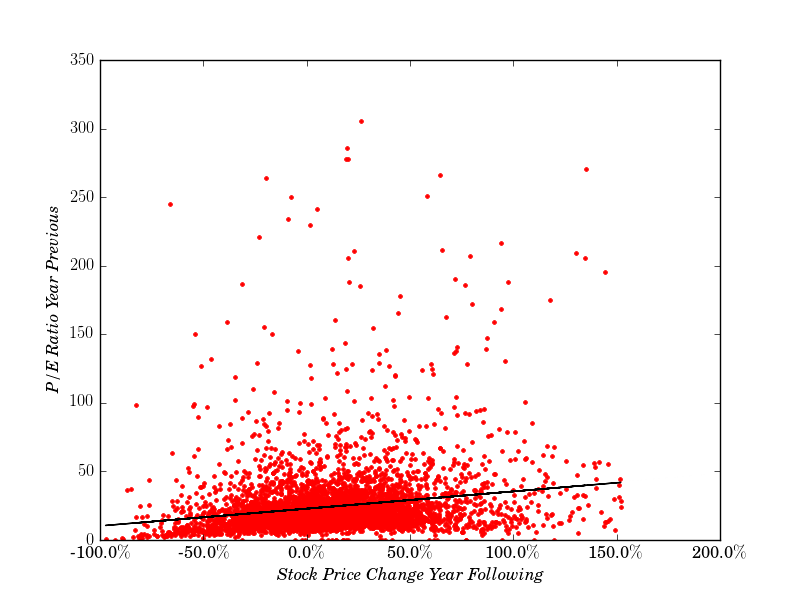
\includegraphics[width=1.2\textwidth]{../work/fundamentals/absolute_pe_ratio_returns.png}}

\section{Attacking the problem - Technical Analysis}
\subsection{Hobbyist Approaches}
\subsection{Review of Metrics}
\subsection{OLMAR algorithm}
\subsection{StatsModels}

\section{Attacking the problem - Machine Learning}
\subsection{KNN on metrics}

\cite {website:pybrain-tutorial}

\bibliography{report}
\bibliographystyle{plainnat}

\end{document}
